\documentclass[12pt]{article}
\usepackage{amsfonts}
\usepackage{booktabs}
\usepackage[margin=1in]{geometry}
\usepackage{amsmath}
\usepackage{gensymb}
\usepackage{cite}
\usepackage{sectsty}
\usepackage{graphicx}
\usepackage{caption}
\usepackage{array}
\usepackage{hyperref}
\usepackage{subfig}
\usepackage{float}
\usepackage{rotating}
\usepackage{tikz}
\usepackage{fixltx2e}
\usepackage{inconsolata}
\usepackage{enumitem}
\usepackage{setspace}
\usepackage[normalem]{ulem}
\newcommand{\msout}[1]{\text{\sout{\ensuremath{#1}}}}
\newcommand\numberthis{\addtocounter{equation}{1}\tag{\theequation}}

\newenvironment{conditions}
  {\par\vspace{\abovedisplayskip}\noindent\begin{tabular}{>{$}l<{$} @{${}={}$} l}}
  {\end{tabular}\par\vspace{\belowdisplayskip}}

\setlength\parindent{0pt}
\usepackage{gensymb}

\begin{document}
\section*{2D Belly Flop Aerodynamic Control}
Rajan Aggarwal\\
December 2020 \\
\noindent\rule{15cm}{0.4pt}

\subsection*{Attitude Control Dynamics}

\begin{figure}[h]
\centering
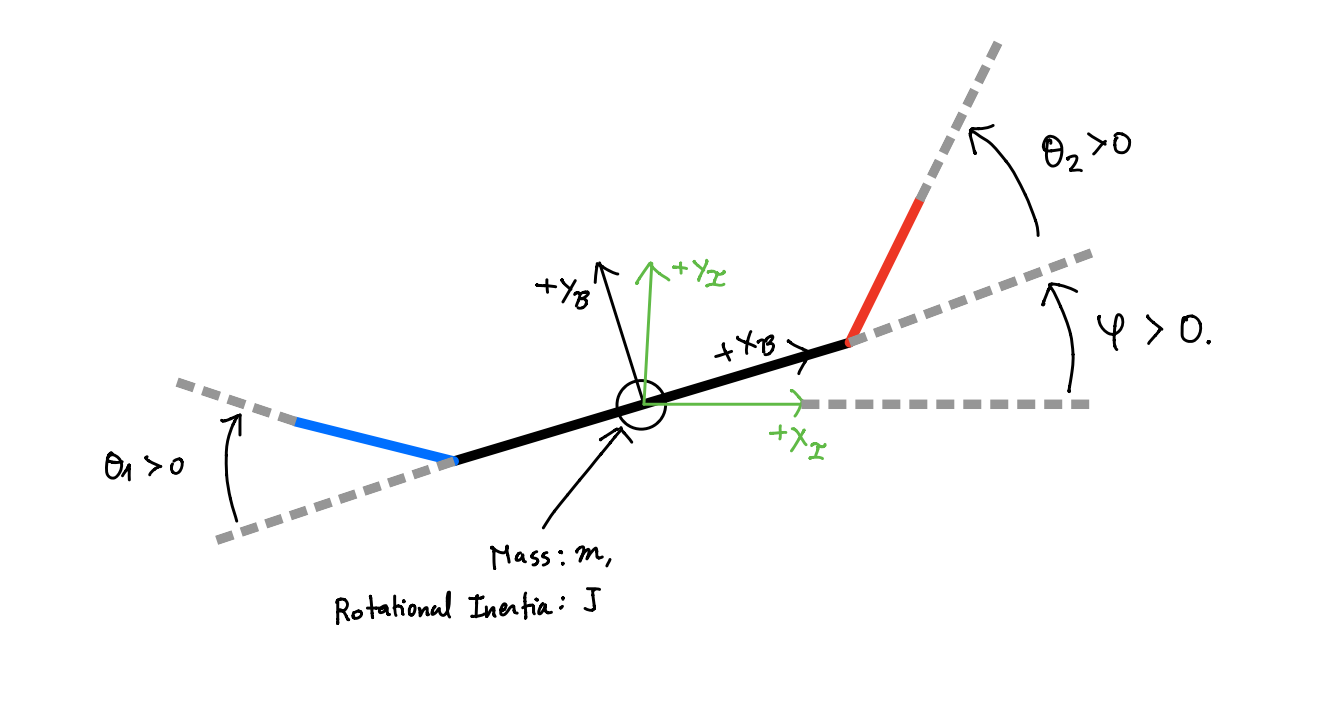
\includegraphics[width=.9\linewidth]{../misc/vehicle_diagram.png}
\caption{Simplified 2D Vehicle Model}
\end{figure}

For the simplified model shown above, which captures the pure roll dynamics and assumes the body is pinned at its center, the equations of motion can be written as follows:

\begin{align*}
\dot{q} &= \frac{d}{dt} q = \frac{d}{dt}\begin{pmatrix}
\varphi \\
\dot{\varphi} \\
\theta_1 \\
\theta_2 \\
\end{pmatrix}
= f(q, u) =
\begin{pmatrix}
\dot{\varphi} \\
\tau_{aero} (\varphi, \theta_1, \theta_2) / J \\
\dot{\theta_1} \\
\dot{\theta_2} \\
\end{pmatrix} \\
\end{align*}

where

\begin{conditions}
q & vehicle state \\
u & control effort, $(\dot{\theta_1}, \dot{\theta_2})^T$ (so we can cost slew rates directly) \\
\varphi & body roll angle [rad] \\
\theta_1 & left flap angle [rad] \\
\theta_2 & right flap angle [rad] \\
\tau_{aero} & aerodynamic torque function acting at body center [N-m] \\
J & rotational inertia of vehicle [kg-m$^2$] \\
\end{conditions}

As the aerodynamic torque is non-linear with respect to the state variables (see sensitivity plots), a local linearization can be used as a start for controller design.  Writing the first order Taylor expansion for $f(q, u)$,

\begin{align*}
f(q, u) \approx f(q_0, u_0) + \frac{\partial f}{\partial q}\Big|_{\substack{q = q_0\\u = u_0}} (q-q_0) + \frac{\partial f}{\partial u}\Big|_{\substack{q = q_0\\u = u_0}} (u-u_0)
\end{align*}

If $(q_0, u_0)$ is chosen to be an equilibrium point -- namely, $f(q_0, u_0) = 0$ -- then the constant term in the Taylor expansion disappears and we have a standard linearized dynamics relation:

\begin{align*}
\dot{q} &= f(q, u) \approx A_{lin} \bar{q} + B_{lin} \bar{u} \\
\end{align*}

with

\begin{conditions}
\bar{q} & $q-q_0$ (state ``error'')\\
\bar{u} & $u-u_0$ (control ``error'')\\
A_{lin} & linear autonomous dynamics Jacobian \\
B_{lin} & linear control dynamics Jacobian \\
\end{conditions}

This formulation can be used in a quadratic-cost, linear-dynamics optimal controller for attitude regulation and tracking (aka, LQR control).

\bigskip\bigskip\bigskip\bigskip
\subsection*{Linear-Quadratic Attitude Controller}

Further expanding out the linear roll dynamics gives:

\begin{align*}
\dot{q} = f(q, u) &\approx A_{lin}\Big|_{\substack{q = q_0\\u = u_0}} \bar{q} + B_{lin}\Big|_{\substack{q = q_0\\u = u_0}} \bar{u} \\
&\approx \begin{pmatrix}
0 & 1 & 0 & 0 \\
\frac{\partial \tau_{aero}}{J \partial \varphi} & 0 & \frac{\partial \tau_{aero}}{J \partial \theta_1} & \frac{\partial \tau_{aero}}{J \partial \theta_2} \\
0 & 0 & 0 & 0 \\
0 & 0 & 0 & 0 \\
\end{pmatrix}\Bigg|_{\substack{q = q_0\\u = u_0}}
\begin{pmatrix}
\varphi - \varphi_0 \\
\dot{\varphi} - \dot{\varphi_0} \\
\theta_1 - \theta_{1, 0} \\
\theta_2 - \theta_{2, 0} \\
\end{pmatrix} +
\begin{pmatrix}
0 & 0 \\
0 & 0 \\
1 & 0 \\
0 & 1 \\
\end{pmatrix}\Bigg|_{\substack{q = q_0\\u = u_0}}
\begin{pmatrix}
\dot{\theta_1} -  \dot{\theta_{1}}_{,0} \\
\dot{\theta_2} -  \dot{\theta_{2}}_{,0} \\
\end{pmatrix}
\end{align*} \\

Note that $\dot{\varphi_0}, \dot{\theta_{1}}_{,0}$ and $\dot{\theta_{2}}_{,0}$ are all $ = 0$ as we restrict linearization points to equilibria points (time derivatives equal to 0). \\

As arbitrary reference values of $\varphi_0, \theta_{1, 0}$ and $\theta_{2, 0}$ are unlikely to result in a moment-equilibrium (due to the underlying constraint of the $\tau_{aero}$ function), we must solve for some of these variables in terms of the others.  Body roll is an intuitive choice for the fixed (desired) variable, leaving the flap angles free.  This results in the system of linear equations:

\begin{align*}
0 &= \tau_{aero}(\varphi_0, \theta_{1, 0}, \theta_{2, 0}) + \begin{pmatrix}
\frac{\partial \tau_{aero}}{\partial \theta_1} & \frac{\partial \tau_{aero}}{\partial \theta_2} \\
\end{pmatrix}\Big|_{\substack{q = q_0\\u = u_0}}
\begin{pmatrix}
\theta_{1, 0} \\
\theta_{2, 0} \\
\end{pmatrix} \\
\end{align*}

With 2 variables and 1 equation (full rank with an extra degree of freedom), opt to use the least-norm solution to find the `feed-forward' $(\theta_1, \theta_2)$ values:

\begin{align*}
\begin{pmatrix}
\theta_{1, 0} \\
\theta_{2, 0} \\
\end{pmatrix}_{ln} &= \begin{pmatrix}
\frac{\partial \tau_{aero}}{\partial \theta_1} & \frac{\partial \tau_{aero}}{\partial \theta_2} \\
\end{pmatrix}^T
\left(\begin{pmatrix}
\frac{\partial \tau_{aero}}{\partial \theta_1} & \frac{\partial \tau_{aero}}{\partial \theta_2} \\
\end{pmatrix}
\begin{pmatrix}
\frac{\partial \tau_{aero}}{\partial \theta_1} & \frac{\partial \tau_{aero}}{\partial \theta_2} \\
\end{pmatrix}^T\right)^{-1}
 (-\tau_{aero}(\varphi_0, \theta_{1, 0}, \theta_{2, 0}))\\
&= \begin{pmatrix}
\frac{\partial \tau_{aero}}{\partial \theta_1} \\
\frac{\partial \tau_{aero}}{\partial \theta_2} \\
\end{pmatrix}
\left(\left(\frac{\partial \tau_{aero}}{\partial \theta_1}\right)^2 + \left(\frac{\partial \tau_{aero}}{\partial \theta_2}\right)^2\right)^{-1}  (-\tau_{aero}(\varphi_0, 0, 0)) \\
&= \frac{-\tau_{aero}(\varphi_0, \theta_{1, 0}, \theta_{2, 0})}{\left(\frac{\partial \tau_{aero}}{\partial \theta_1}\right)^2 + \left(\frac{\partial \tau_{aero}}{\partial \theta_2}\right)^2}
\begin{pmatrix}
\frac{\partial \tau_{aero}}{\partial \theta_1} \\
\frac{\partial \tau_{aero}}{\partial \theta_2} \\
\end{pmatrix} \\
\end{align*}

The moment-balance least norm solution solves for $(\theta_{1, 0}, \theta_{2, 0})^T$, but requires a linearization about $(\theta_{1, 0}, \theta_{2, 0})^T$ in the evaluation of $(\frac{\partial \tau_{aero}}{\partial \theta_1} , \frac{\partial \tau_{aero}}{\partial \theta_2})$, as well as knowledge of $(\theta_{1, 0}, \theta_{2, 0})^T$ to evaluate $\tau_{aero}$ -- circular references.  The gradients as a function of pose are numerically compliant about the points we're interested in, so in this case it's acceptable as a first-pass to evaluate them at a nearby (known) fixed equilibrium point (e.g. $\varphi = \theta_1 = \theta_2 = 0$) and assume those gradients hold for the reference position we solve for: $(\varphi_{0}, \theta_{1, 0}, \theta_{2, 0})$.  For completeness, one could execute an iterative approach: a) evaluate the torque and gradients at a nearby fixed equilibrium point, b) solve for a new reference pose ($\varphi_{0}, \theta_{1, 0}, \theta_{2, 0}$)$^T$ using those values, c) re-evaluate the DC torque and gradients at this new reference pose, and repeat until convergence within an L2 norm change of $<\epsilon$ between $(\varphi_{0}, \theta_{1, 0}, \theta_{2, 0})_{i}^T$ and $(\varphi_{0}, \theta_{1, 0}, \theta_{2, 0})_{i+1}^T$.  This amounts to a mini-optimization problem of sorts over the $\tau_{aero}$ function -- there are probably more principled ways to do this.  A visualization of the `zero moment' surface embedded in the 3D pose-space is shown below:
\clearpage

\begin{figure}[h!]%
    \centering
    \subfloat[\centering View 1]{{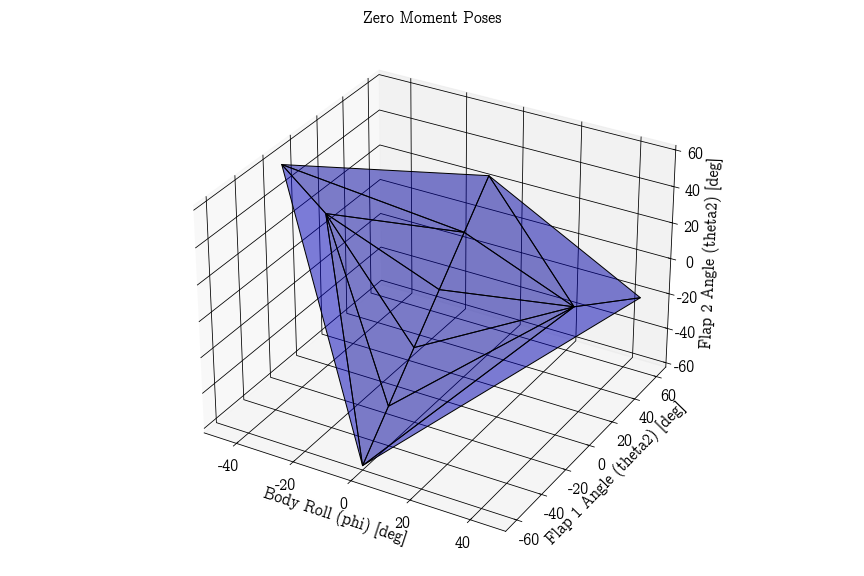
\includegraphics[width=.45\linewidth]{../misc/zero_moment_poses_view1.png} }}%
    \qquad
    \subfloat[\centering View 2]{{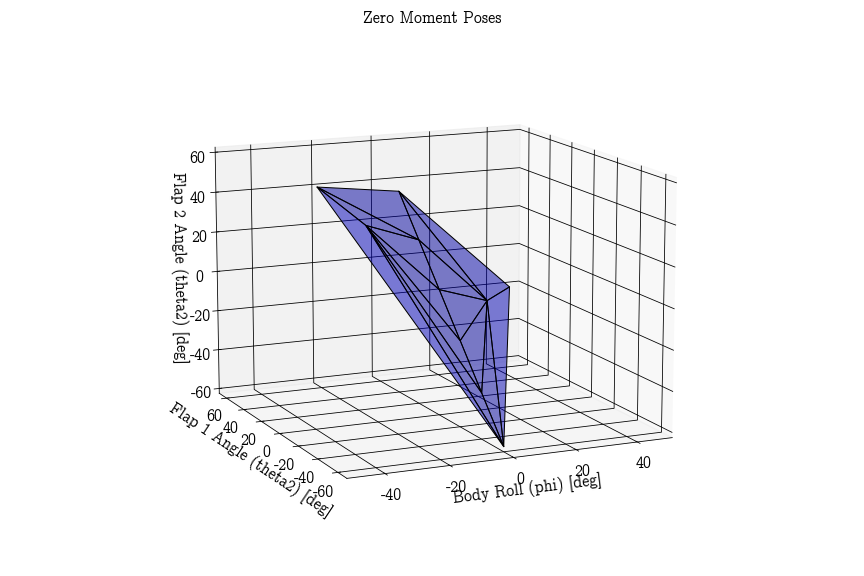
\includegraphics[width=.45\linewidth]{../misc/zero_moment_poses_view2.png} }}%
    \caption{Zero moment surface in the pose space.  For a given desired body roll value, $\theta_{1}$ and $\theta_{2}$ are constrained to lie on the slice of this surface at $\varphi_{0}$.  The least norm solution for $\theta_{1}$ and $\theta_{2}$ can be visualized as dilating a circle from the $(\varphi = \varphi_{0}, \theta_{1} = \theta_{2} = 0)$ point in the $\varphi = \varphi_{0}$ plane until the circle becomes tangent with the manifold.  As an intuition-check, when $\varphi = 0$, the locus of zero-moment $(\theta_1, \theta_2)$ pairs is simply a 1:1 line, which defines a family of symmetric V-shaped poses.}
    \label{fig:example}%
\end{figure}


With this extension of the linear dynamics, the problem is now well-posed for optimal control -- in this case, an infinite-horizon LQR:

\begin{align*}
\underset{\bar{u}(t)}{\text{min}} \, J(\bar{q}(t), \bar{u}(t)) &= \int_0^\infty (\bar{q}^T Q \bar{q} + \bar{u}^T R \bar{u}) \, dt \\
\text{subject to} \,\,\, \frac{d}{dt}\bar{q} &= A_{lin} \bar{q} + B_{lin} \bar{u} \\
\end{align*}

where $Q$ and $R$ are weight matrices that penalize spending time in the closed-loop trajectory that are far from the desired reference pose and reference command effort, respectively.  \\


The solution to this optimal problem is analytical and well-known -- one such solution is to solve the continuous-time algebraic Ricatti equation for $P$:

\begin{align*}
0 &= A^T P + PA - PBR^{-1}B^T P + Q
\end{align*}

and then construct the feedback policy using $P$ as

\begin{align*}
\bar{u}_{LQR}(t) &= -R^{-1}B^T P \bar{q}(t)
\end{align*}


With this control law, the closed-loop dynamics then becomes:

\begin{align*}
\frac{d}{dt}\bar{q} &= (A_{lin} - BR^{-1}B^T P) \bar{q}(t) \\
&= A_{cl}\bar{q}(t) \\
\end{align*}

Which can be analyzed and simulated as an autonomous linear system. \\

Simulation can also be done non-linearly, to test the validity of the local aerodynamics linearization and to incorporate various other real-world model mismatches (e.g. friction, actuator time delays, probabilistic disturbances, etc.) \\

An LQR reference-tracking control with some aerodynamics non-linearities included in the closed loop was simulated in \texttt{AttitudeController.py}, with signal traces below (see repo for an animation and code):


\begin{figure}[h]
\centering
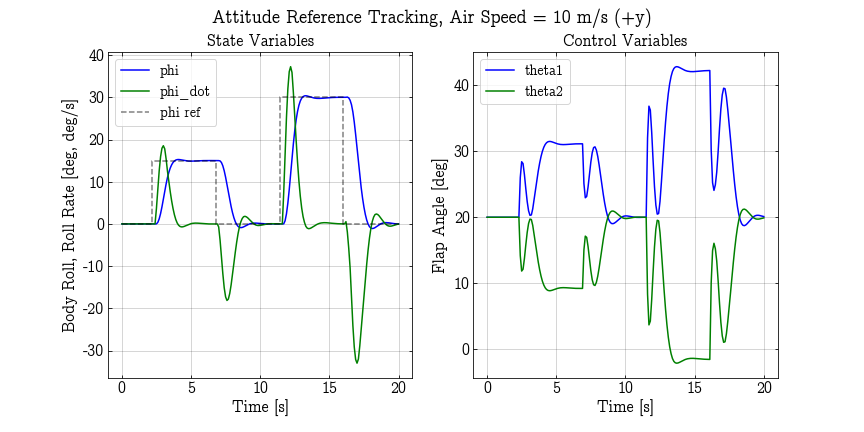
\includegraphics[width=.9\linewidth]{../control_figures/attitude_ref_tracking.png}
\caption{LQR control in closed-loop}
\end{figure}



\bigskip\bigskip\bigskip\bigskip
\subsection*{Non-linear Trajectory Optimization, Open-Loop}

For fun, also tried taking this 2D model to calculate single-shot open-loop optimal trajectories for a pin-point landing maneuver (opening up the dynamics to cross-range and altitude dynamics).  The state vector expands and takes the following form:

\begin{align*}
\dot{q} &= \frac{d}{dt} q = \frac{d}{dt}\begin{pmatrix}
X \\
\dot{X}\\
Y \\
\dot{Y} \\
\varphi \\
\dot{\varphi} \\
\theta_1 \\
\theta_2 \\
g \\
\end{pmatrix} =
f(q, u) =\begin{pmatrix}
\dot{X} \\
K_{aero}(\frac{\partial F_x}{\partial \varphi} + \frac{\partial F_x}{\partial \theta_1} +\frac{\partial F_x}{\partial \theta_2})/m \\
\dot{Y} \\
K_{aero}(\frac{\partial F_y}{\partial \varphi} + \frac{\partial F_y}{\partial \theta_1} +\frac{\partial F_y}{\partial \theta_2})/m + F_{y, const}/m - g/m \\
\dot{\varphi} \\
K_{aero}(\frac{\partial M_z}{\partial \varphi} + \frac{\partial M_z}{\partial \theta_1} +\frac{\partial M_z}{\partial \theta_2})/J \\
\dot{\theta_1} \\
\dot{\theta_2} \\
0\\
\end{pmatrix} \\
\end{align*}

where

\begin{conditions}
X & inertial x-coordinate (cross range) [m] \\
Y & inertial y-coordinate (altitude) [m] \\
g & gravitational accel = 9.81 [m/s$^2$], included for possible linearization later \\
F_{y, const} & constant (DC) drag term about linearized aerodynamics pose \\
m & vehicle mass [kg] \\
K_{aero} & vehicle velocity aerodynamic load scaling factor [-] \\
\end{conditions}

A constant drag force in $Y$ is included in the dynamics, but equivalent forces are not needed for $X$ and $\varphi$ (this is because about the aerodynamics linearization point with symmetric flaps, there are no aero loads in $X$ or in torque about $Z$).  To improve performance one could put these dynamics into a nicer (fully linear) form, but for now is kept as is. \\

A $K_{aero}$ term is utilized as well which scales the aerodynamic loading factors via a square-law on the $Y$ velocity -- this is to account for the fact that the CFD sims were run at a constant velocity of 10 m/s, whereas in this simulation the vehicle can be expected to deviate from that air stream velocity (and we wouldn't want the vehicle to be able to build a positive velocity in $Y$!) \\

The optimal trajectory problem can be formulated as a minimum-time, minimum-roll rate, minimimum-actuator effort, minimum-state error etc., or some combination thereof (lots of possibilities).  It is important to keep the dynamics and constraints as `well-behaved' (convex) as possible, to enable efficient solve times and feasible optimizations.  In \texttt{HorizonOptimization.py}, a stage-wise cost of time, roll rate and actuator slews was used to find a minimal-cost trajectory, with convex constraints on actuator limits and body configurations.  The horizon was temporally discretized into $N = 50$ points with RK4 integration to stitch the discrete dynamics together.  CasADi with an interior-point solver (IPOPT) was used to solve the non-linear program.  Below, a sample optimal trajectory is shown starting at $(X, Y) = (100, 100)$ and landing at the origin (animation and figure are in the repo as well):
\clearpage

\begin{figure}[h]
\centering
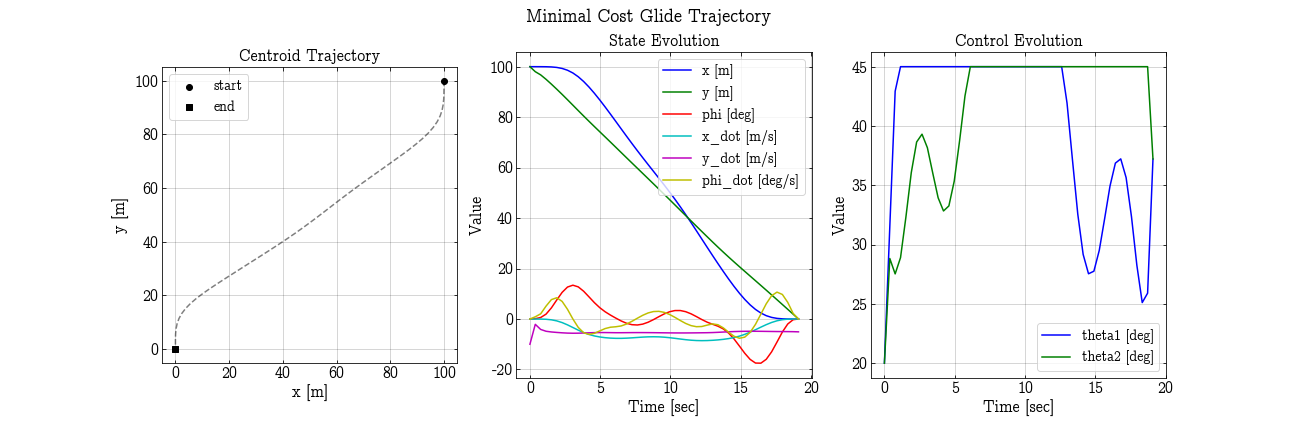
\includegraphics[width=1.0\linewidth]{../control_figures/minimal_cost_trajectory.png}
\caption{Minimal-cost open-loop trajectory}
\end{figure}


As this optimization is open-loop, simply executing the optimal $\bar{u}_i 's$ would not result in the clean trajectory shown above, as there is no feedback that regulates error that arises due to process and environment model mismatch.  In practice, solving such an optimization is only useful in a receding-horizon formulation, where: the optimal trajectory is solved very quickly (relative to the time-constants of the dynamics), the first few steps on that trajectory are taken, and then a new trajectory is solved that takes into account the current location of the system in its state- and control-space.  This adds in a closed-loop nature to the control, imbuing it with some robustness to model and environmental mismatch.  This area of research is quite rich and there's a lot of work that goes into the dynamics formulation, optimization problem structure, and recursive feasibility/stability of the whole paradigm, and is classically published under names like Model-Predictive Control (MPC) or Receding-Horizon Control (RHC).  Often times too one can find these longer-term predictive controllers cascaded with shorter-term feedback controllers to improve performance.  There's a \textit{lot} more that one could do in this example with respect to improving performance and robustness in a model-predictive controller, but for now I'll leave it here as an exercise in exploration.


\bigskip\bigskip\bigskip\bigskip
\subsection*{Aerodynamic Loads Simulation}

For the vehicle model shown in Figure 1, a suite of computational fluid dynamics (CFD) simulations were run to evaluate forces ($F_x, F_y$) and moments ($M_z$) on the body as a function of its roll and flap angles (this is the basis of the $\tau_{aero}$ function and other gradients referenced in the above controllers). The dimensions were scaled to something that could be constructed as a hobby project (see next section), so all-in-all the vehicle dimensions are bounded by $\sim$ 0.5 x 0.5 x 1.0 m.  Standard temperature and pressure incoming air was used, with a stream velocity of 10 m/s in Inertial $Y+$.  As a first run, a fully-outstretched configuration ($\varphi = \theta_1 = \theta_2 = 0$) was simulated to back-check with flat-plates-in-flow formulas in introductory fluid mechanics textbooks:

\clearpage

\begin{figure}[h!]
\centering
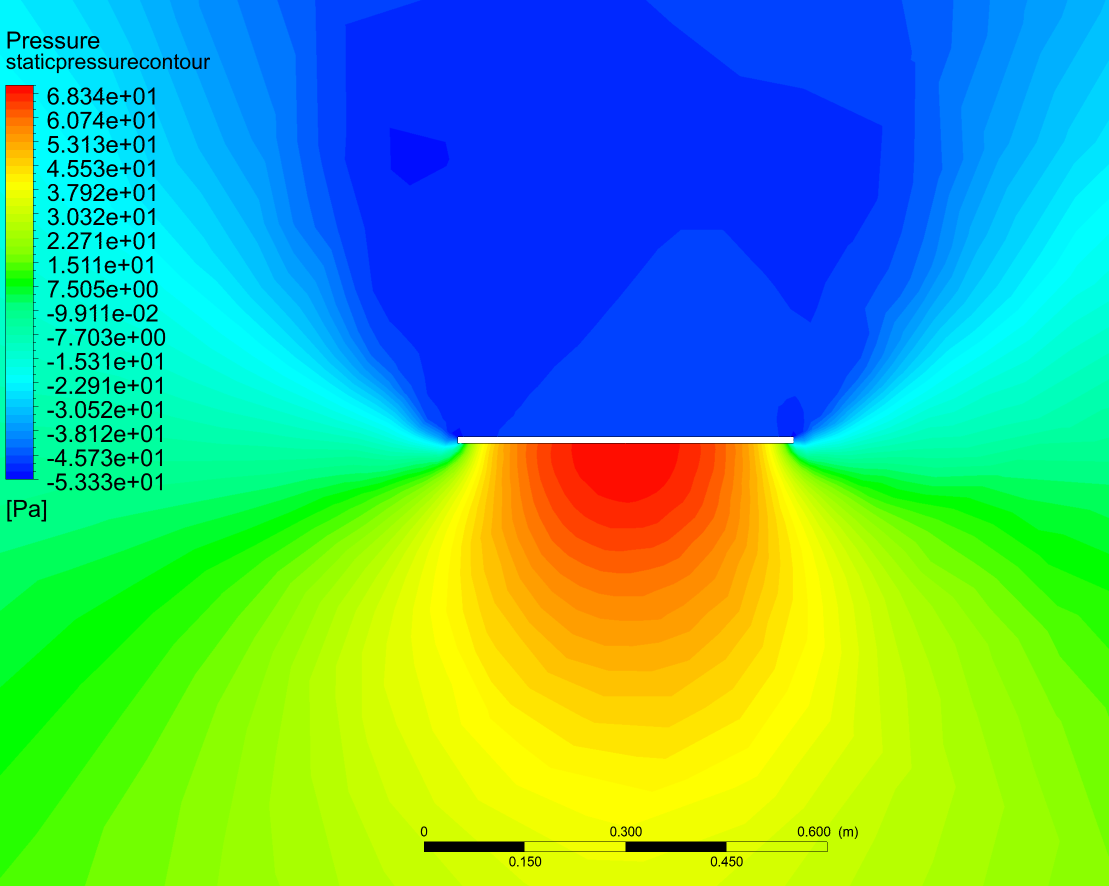
\includegraphics[width=.6\linewidth]{../cfd_figures/flat_config_static_pressure.png}
\caption{Static Pressure, $\varphi = \theta_1 = \theta_2 = 0$}
\end{figure}

The drag force predicted by the textbooks is:

\begin{align*}
F_D &= \frac{1}{2} \rho C_D A v^2 \\
&= \frac{1}{2} (1.225 \, \text{kg/m$^3$}) (2.0) (.50 \, \text{m$^2$}) (10. \, \text{m/s})^2 \\
&\approx 60. N \\
\end{align*}

where CFD calculated 51 N.  So not bad. \\

With this in mind a larger parameter study was conducted, with the following analysis grid (n = 196 cases total, symmetry in the $\varphi$ results was leveraged to reduce test points):

\begin{align*}
\varphi &\in \{-45, -30, -15, 0, +15, +30, +45\} \, \text{deg} \\
\theta_1 &\in \{-60, -40, -20, 0, +20, +40, +60\} \, \text{deg} \\
\theta_2 &\in \{-60, -40, -20, 0, +20, +40, +60\} \, \text{deg} \\
\end{align*}

Some interesting configurations for $\varphi = 0$ are shown below:
\clearpage

\begin{figure}[h!]
\centering
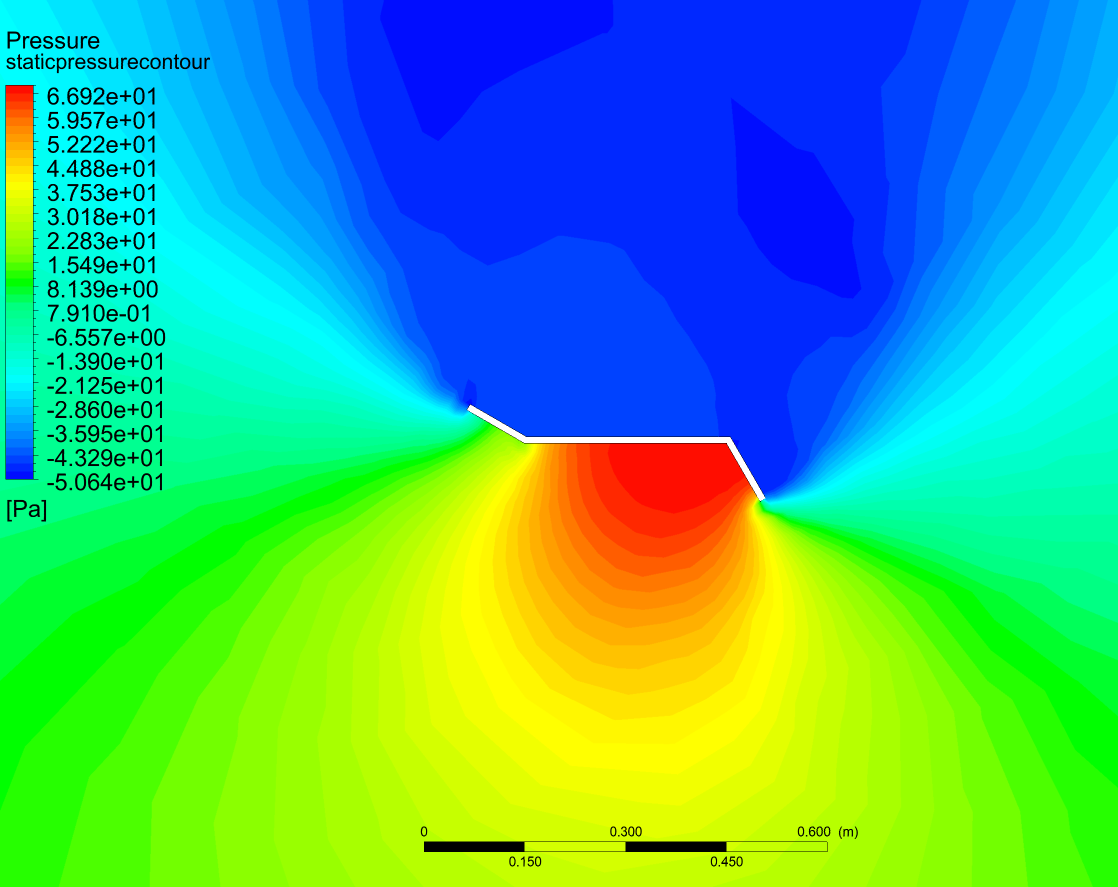
\includegraphics[width=.6\linewidth]{../cfd_figures/max_fx_config_static_pressure.png}
\caption{Static Pressure, Max Fx configuration}
\end{figure}

\begin{figure}[h!]
\centering
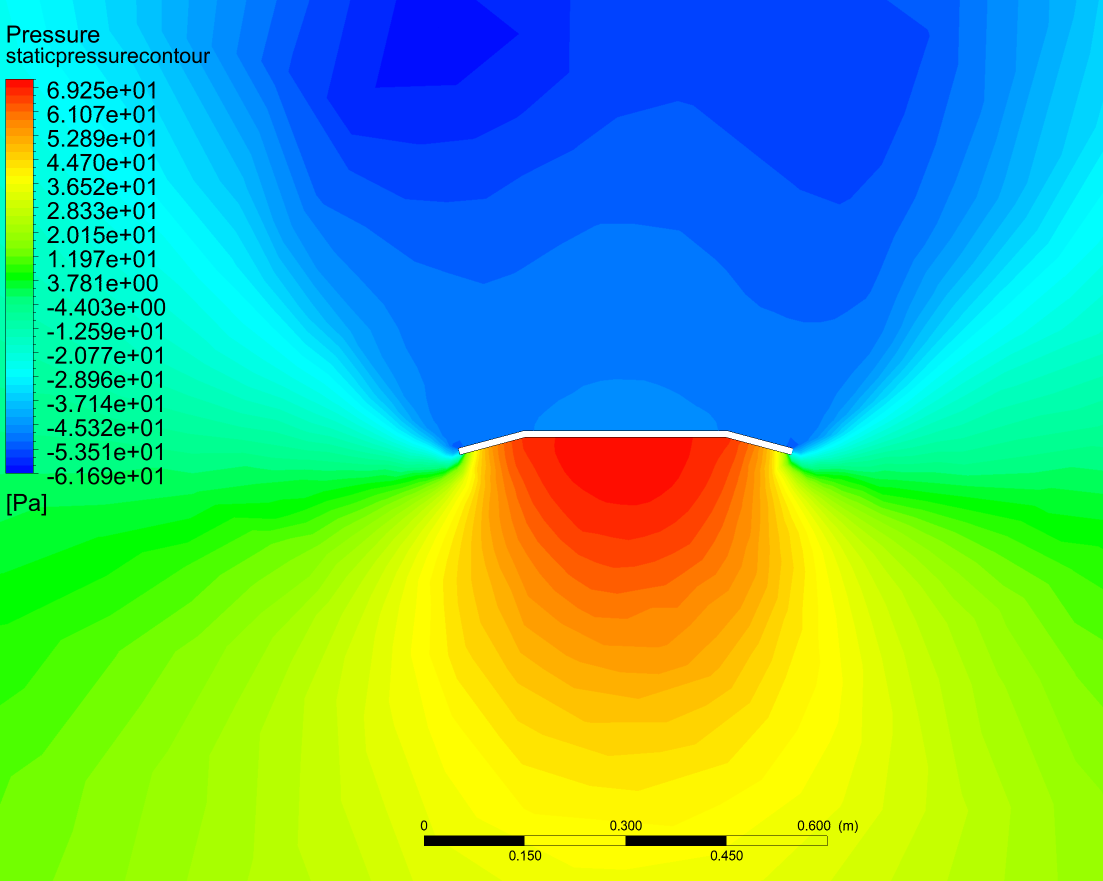
\includegraphics[width=.6\linewidth]{../cfd_figures/max_fy_config_static_pressure.png}
\caption{Static Pressure, Max Fy configuration (slight `cupping' into the flow)}
\end{figure}

\clearpage

\begin{figure}[h!]
\centering
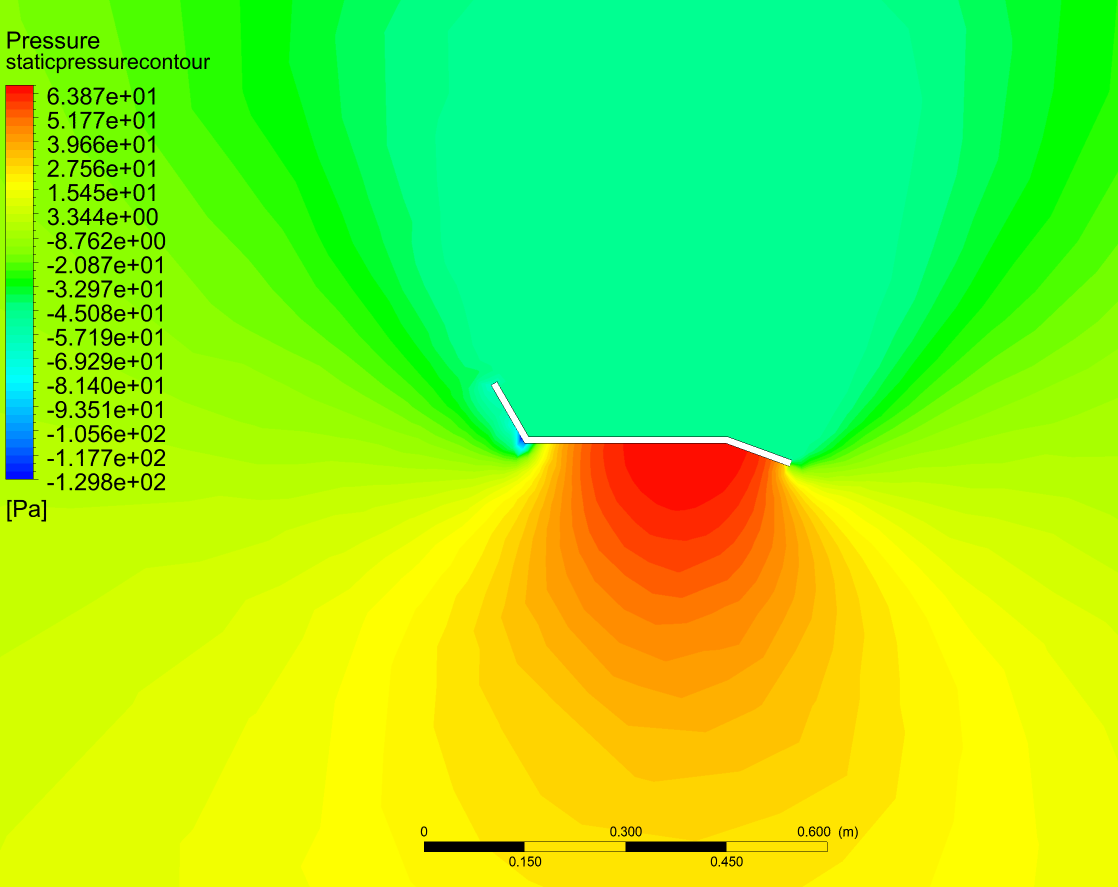
\includegraphics[width=.6\linewidth]{../cfd_figures/max_mz_config_static_pressure.png}
\caption{Static Pressure, Max Mz configuration}
\end{figure}

Using these results, a set of sensitivity plots can be generated which show visually how the loads change as a function of $\varphi, \theta_1 \, \text{and} \, \theta_2$ (see repo for full-sized images):

\begin{figure}[h!]
\centering
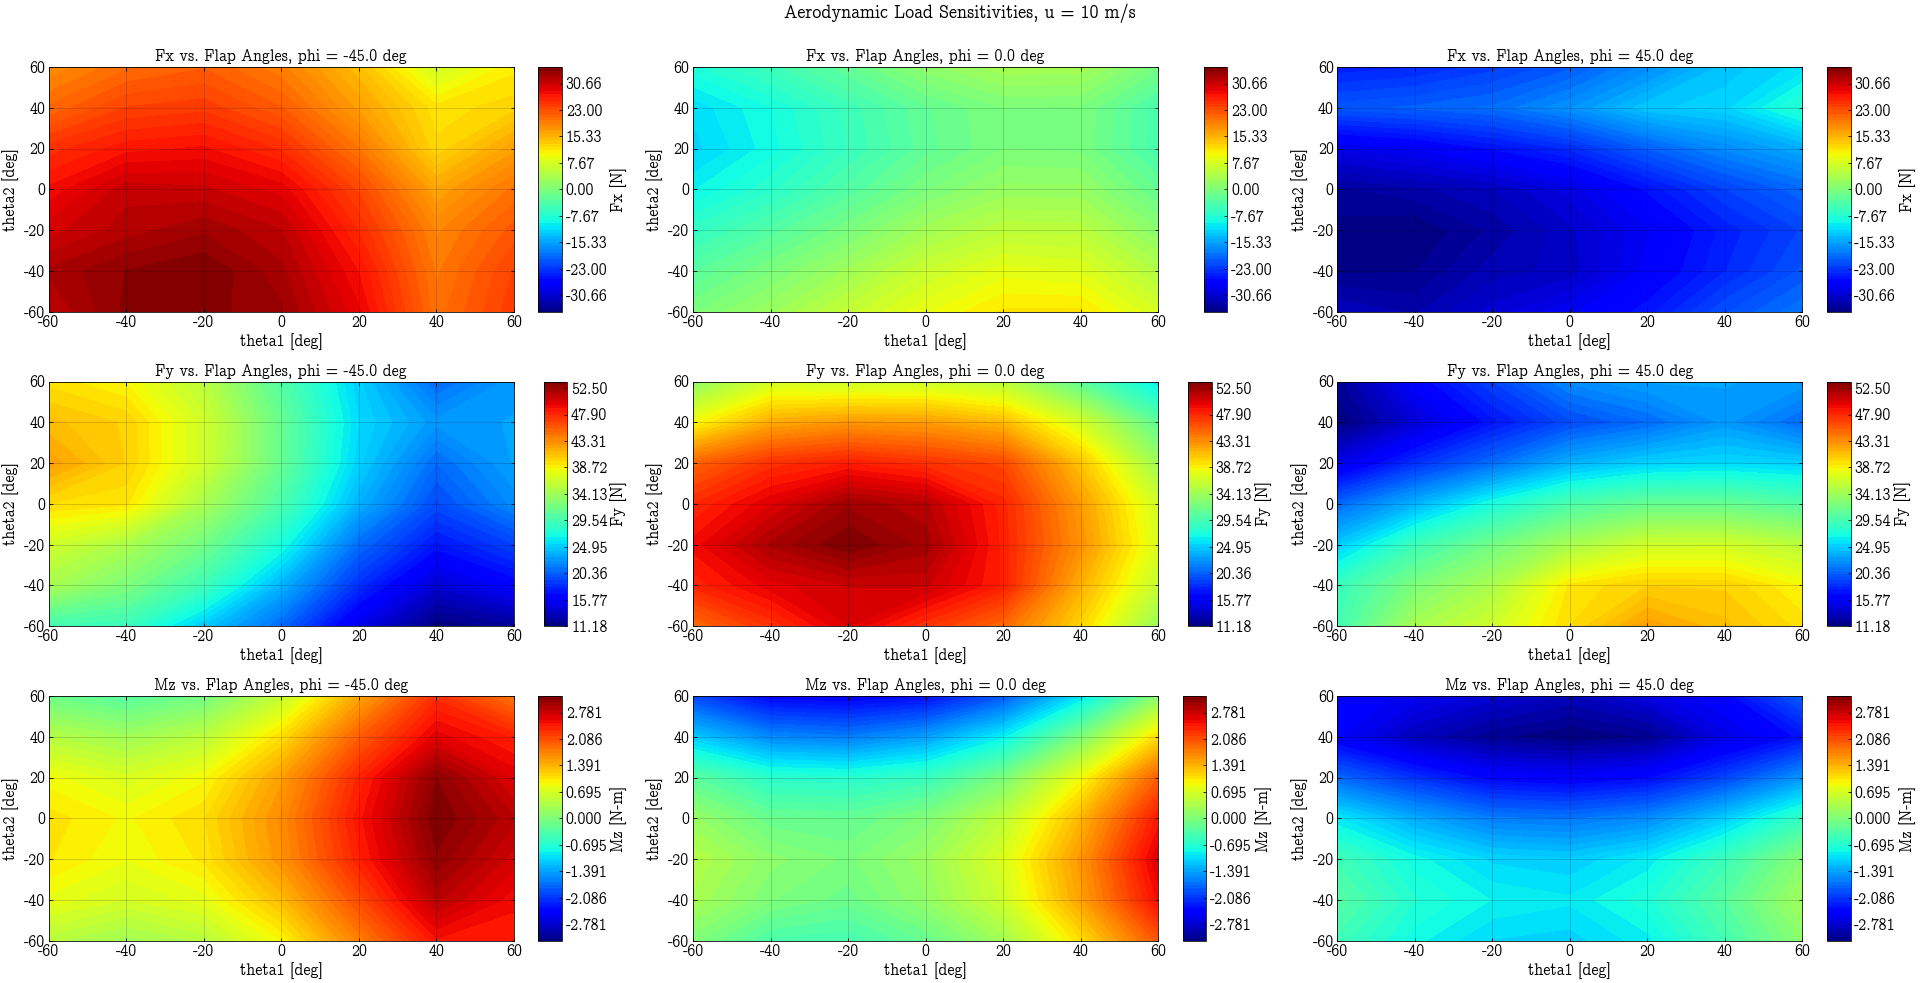
\includegraphics[width=1.0\linewidth]{../cfd_parameter_study/full_aero_load_sensitivities.png}
\caption{Full CFD Aerodynamic Load Sensitivities.  Colorbars are consistent row-wise, to better illustrate the strengths of 2nd order trends, like saddle points.}
\end{figure}


It is ultimately this non-linear function that is interpolated and finite-differenced to collect the aerodynamic sensitivities used in the linearized dynamics above (see \texttt{AeroSensitivityAnalyzer.py} for more).


\bigskip\bigskip\bigskip\bigskip
\subsection*{Possible Build Project}

The above dynamics, controllers and CFDs were simulated with the thought of perhaps building this as a hobby project one day:

\begin{figure}[h!]
\centering
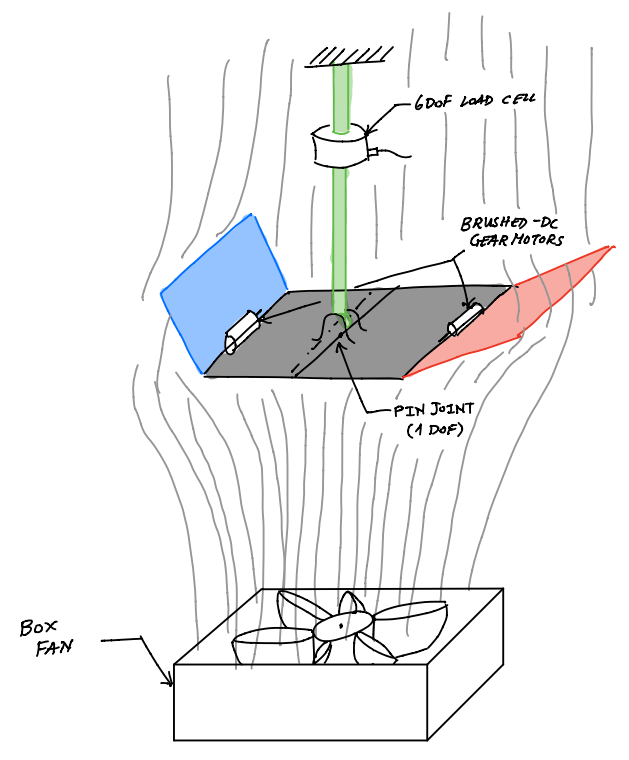
\includegraphics[width=.6\linewidth]{../misc/testbed_figure.png}
\caption{A possible testbed, using a box fan to generate aerodynamic forces.}
\end{figure}

The idea would be to use a pin joint to constrain the vehicle in all degrees of freedom except roll, and modulate the flaps with gearmotors to generate differential aerodynamic torque with feedback on a central IMU.  Without the 6 DOF load cell, the overall build could be relatively low-budget.  But, with the 6 DOF load cell, one could run a separate, real-time non-linear simulation that forward-propagates the loads in a 2D virtual environment, to position the vehicle in (X,Y) space.  This position could then be fed into the controllers that try to regulate position and perform a pin-point landing (the controllers \textit{think} the vehicle is flying through 2D space, but in reality it's pinned to a post).  With this non-linear simulation up and running one could then inject artificial disturbances, controller delays, model mismatches, actuator-out cases etc. to test the robustness of the system with hardware-in-the-loop.

\end{document}